\documentclass[tikz,border=5pt]{standalone}
\usepackage{luatexja}
\usepackage[hiragino-pron]{luatexja-preset}
\usepackage{amsmath,amssymb}
\usepackage{pgfplots}
\pgfplotsset{compat=1.18}
\usetikzlibrary{arrows.meta,calc,decorations.markings,patterns,positioning}

% Common styles
\tikzset{
  axis/.style={-{Stealth[length=6pt]}, thick},
  curve/.style={thick, red},
  dashed curve/.style={thick, dashed, blue},
  dot/.style={circle, fill, inner sep=1.5pt},
  open dot/.style={circle, draw, fill=white, inner sep=1.5pt},
}

\begin{document}
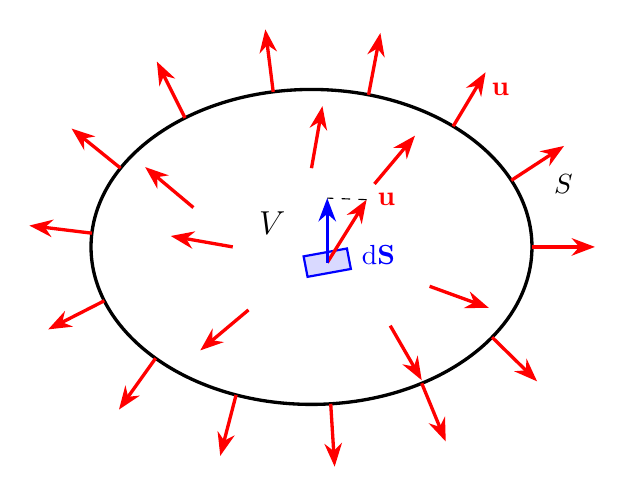
\begin{tikzpicture}[>=Stealth, thick]

  % Closed surface S (elongated ellipse)
  \draw[very thick] (0,0) ellipse (2.8 and 2.0);

  % Red outward arrows at points around the ellipse
  \foreach \angle in {0,25,...,335} {
    \pgfmathsetmacro{\px}{2.8*cos(\angle)}
    \pgfmathsetmacro{\py}{2.0*sin(\angle)}
    % Normal direction for ellipse: (x/a^2, y/b^2) normalized, scaled to length 0.8
    \pgfmathsetmacro{\nx}{cos(\angle)/2.8}
    \pgfmathsetmacro{\ny}{sin(\angle)/2.0}
    \pgfmathsetmacro{\norm}{sqrt(\nx*\nx+\ny*\ny)}
    \pgfmathsetmacro{\nx}{0.8*\nx/\norm}
    \pgfmathsetmacro{\ny}{0.8*\ny/\norm}
    \draw[->, red, very thick] (\px,\py) -- ++(\nx,\ny);
  }

  % Red arrows inside the volume (divergence field)
  \foreach \x/\y/\ang in {
    -1.5/0.5/140, -0.8/-0.8/220, 0.8/0.8/50,
    1.5/-0.5/340, 0.0/1.0/80, -1.0/0.0/170,
    1.0/-1.0/300
  }{
    \draw[->, red, very thick] (\x,\y) -- ++(\ang:0.8);
  }

  % u label near top-right arrow
  \node[red] at (2.4,2.0) {$\mathbf{u}$};

  % V label inside
  \node at (-0.5,0.3) {\large $V$};

  % Blue dS: parallelogram + normal vector
  \coordinate (P) at (0.2,-0.2);
  \coordinate (dA) at (-0.25,-0.18);
  \coordinate (dB) at (0.3,-0.08);
  \fill[blue, opacity=0.15]
    ($(P)+(dA)$) -- ($(P)+(dB)$) -- ($(P)-(dA)$) -- ($(P)-(dB)$) -- cycle;
  \draw[blue, thick]
    ($(P)+(dA)$) -- ($(P)+(dB)$) -- ($(P)-(dA)$) -- ($(P)-(dB)$) -- cycle;
  % Red arrow: u at P, tilted so that its normal component = blue vector
  % Blue vector direction: (0.15, 0.8), add tangential offset (0.5, -0.09375) to keep normal component
  \draw[->, red, very thick] (P) -- ++(0.5,0.8) node[right] {$\mathbf{u}$};
  % Dashed projection
  \draw[dashed, thin] ($(P)+(0.5,0.8)$) -- ($(P)+(0,0.82)$);
  % Blue arrow: normal component of u
  \draw[->, blue, very thick] (P) -- ++(0,0.82);
  \node[blue] at (0.85,-0.1) {$\mathrm{d}\mathbf{S}$};

  % S label
  \node at (3.2,0.8) {$S$};

\end{tikzpicture}
\end{document}
